\section{La méthodologie}
La qualité du logiciel \FactDev{} est principalement dû à la rigueur dans l'application de la méthodologie de développement. 

Elles fûrent définies en même temps que la conception du logiciel durant le \Sprint{} \textit{0}. Cela comprend les attitudes à adopter par les membres de l'équipe sur le plan organisationnel et techniques avec le respect de conventions qui ont aussi été défini à ce moment là.
 
\subsection{Le respect de la méthode Scrum}
Au niveau de la gestion du développement par la méthode \Scrum{} nous avons tenu un \Backlog{} \ref{backlog}. Dans celui-ci se trouve l'ensemble des \UserStories{} et\TechnicalStories{} que nous avions à réaliser durant le projet. Ces \Stories{} ont été déterminée lors de \PlanningPoker durant les mêlées. C'est durant ces séances que nous déterminions le poids attribué à chacune des \Stories{} et comment les répartir sur les six \Sprints{} des deux \Releases.  

La répartition des \Stories{} s'est faite en fonction de leur poids mais aussi en tenant compte de l'équipe et des événements pouvant survenir. Ainsi le premier \Sprint{} été plutôt léger car il tenait compte du temps d'apprentissage du langage C++ et du framework Qt. Les autres \Sprints{} sont en revanche équilibré. Les deux derniers sont également plus léger sur le plan technique car nous voulions consacrer du temps à la rédaction des documents et à la préparation de la soutenance. De plus, certaines tâches possédaient un fort taux d'inconnu et il était donc difficile de lui attribuer un poids. 
  
Lorsque nous ne pouvions nous voir pour assurer les mêlées quotidiennes, nous nous retrouvions sur une zone  de chat \textit{« \#irc »} que nous avions créé pour la circonstance. Ainsi, nous faisions le point sur l'évolution du projet et débattre sur des choix de conception.

L'assiduité et le respect de la méthode \Scrum{} est visible sur le \Github{} de notre projet. En effet, le nombre de \PullRequest{} (95), d'\Issues{} (145), de branches (91) et de \Commits{} (près de 1200) en est une preuve. Les \PullRequest{} mettent également en avant la communication entre les membres de l'équipe.

Autre preuve de notre implication dans le respect de cette méthode, le \BurnUp{} ci-dessous: 
\begin{figure}[H]
	\centering
	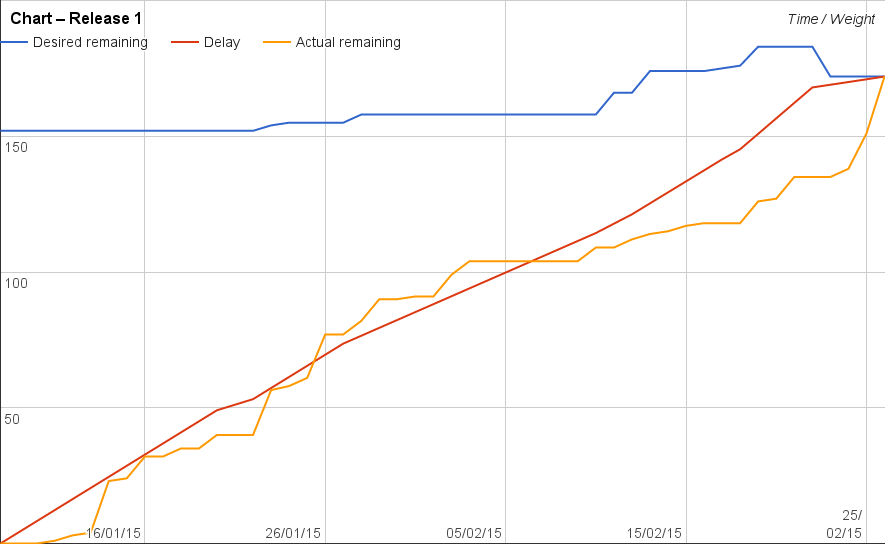
\includegraphics[width=14cm]{screens/release1-chart.png}
	\caption{Burn Up chart de la première release}
	\label{fig:burnupchart-release1}
\end{figure}
La courbe rouge représente l'évolution théorique du projet durant les \Sprints{} de la première \Release. On constate que notre avancé (courbe orange)  suit globalement la courbe théorique. Cependant, l'on observe une baisse de notre activité durant la semaine du 5 février qui correspondait à notre période de vacance. De plus, on note également que lors du \Sprint{} 3 nous nous sommes trouvés en dessous de l'objectif. Cela s'explique par une augmentation du nombre de \Stories{} (courbe bleu) qui correspondait à des modifications ergonomiques où à la résolution de bugs. Certaines d'entre-elles étaient sujet à discussion et ont donc été reportées au \Sprint{} d'après. Néanmoins nous sommes parvenus à finir nos \Sprints{} dans les temps. 

Chacun des \Sprints{} a été réalisé dans les temps et fut l'objet d'une démonstration auprès de M. \bsc{Migeon}. 

\subsection{Les outils de qualité du code}
La qualité du code peut être mesurer grâce à différents outils. 

Dans notre cas nous avons utilisé plusieurs outils tel que \Travis{} pour l'intégration continue, \Coveralls{} pour la couverture de code ou encore \SonarQube{} qui fournit des informations diverses sur le code (nombre de lignes de code, respect des convention de nommage, niveau de complexé, duplication du code). 

\Travis{} nous a permis de s'assurer que le logiciel compile sur une machine tierce, que les tests unitaires passent et de mettre à jour nos documents (manuel d'utilisateur ou \textit{Doxygen}). Associé à \Github{} l'on sait après chaque \Commit{} si le \Build{} passe. C'est également lui qui fournit à \Coveralls{} notre code à analyser pour vérifier la couverture de notre code. De plus, le fait que l'on ne peut pas intégrer notre code si la couverture de code régresse nous oblige à faire des tests unitaires sur les nouvelles fonctionnalités que l'on a implémenté. Ainsi, à la fin de notre projet, la couverture de code est de 90\%. Cette continuité dans l'implémentation des tests unitaires nous a permis de faire du \Refactoring{} régulièrement sans crainte de provoquer des régressions du logiciels. Cela a été particulièrement efficace lors de l'ajout d'un second système de gestion de base de données où l'on devait s'assurer que les méthodes fonctionnent aussi bien sur un système que sur l'autre.  


